\documentclass[11pt]{exam}

\usepackage{listings}
\lstset{basicstyle=\footnotesize, showstringspaces=false,columns=fullflexible, basicstyle=\footnotesize\ttfamily, frame=tb }
\usepackage{pdfsync}
\usepackage{subfigure}
\usepackage{amsmath}
\usepackage{amsfonts}
\usepackage[pdftex]{graphicx}
\usepackage{enumitem}
\usepackage{fullpage}
\usepackage{wrapfig}
\usepackage[small]{caption}

\setlength{\parindent}{0in} % Removing indentation of new paragraphs

\title{Status Report}
\author{Mads Hartmann Jensen}

\begin{document}

\maketitle{}

\paragraph{} This report contains the details of my work for Hannes on his PhD project Kopitiam during my employment. The purpose is not to explain the theory behind the work but rather give an overview of what I've worked on and the state of completion as I leave the project. the My work includes build system setup and different kinds of static analysis of Java programs. \newline \newline

\newpage

\tableofcontents

\newpage

\section{Build System}

I switched the build system of the project to use the popular Scala build tool SBT (Simple Build Tool) and set up support for automated tests and automatic test coverage reports.

\section{Live variable analysis}

I implemented a live variable analysis of Java programs. The goal of the analysis is to remove any dead variables introduced by our conversion from Java to Simple Java rather then attempt to improve the original Java programs written by the user of Kopitiam.

\subsection{Details}

The implementation can be found in the file \texttt{src/main/scala/dk/itu/sdg/analysis/Optimizer.scala} and the tests can be found in \texttt{src/test/scala/dk/itu/sdg/analysis/OptimizerTest.scala}. \newline

TODO: Write a little about the data-structures and high-level algorithm.

\subsection{State of Completion}

TODO: I'll write this when the two last tests pass.

\newpage

\section{Purity analysis}

I've implemented a Purity analysis of Java programs based on the paper
A Combined Pointer and Purity Analysis for Java Program by Alexandru
Salcianu and Martin Rinard. I also presented the algorithm to the
Tools and Methods for Scalable Software Verification (TOMESO) group at
ITU.

\subsection{High Level Algorithm}

\subsubsection*{Data}

For each method a points-to graph is constructed; the points-to graph
consists of a set of nodes, a set of edges, the state of the local
variables and a set of globally escaped nodes. The \textbf{nodes}
model heap objects and can be of the following types:

\begin{itemize}
  \setlength{\itemsep}{1pt}
  \setlength{\parskip}{0pt}
  \item \emph{Inside Nodes} model the objects created by the analyzed method
  \item \emph{Outside Nodes} model the objects that are passed as arguments 
        to the method
  \item \emph{Parameter Nodes} model the objects read from outside the method
\end{itemize}

The \textbf{edges} of the graph are used to model heap references. I will use
$<n1,f,n2>$ to denote an edge from n1 to n2, labeled with the field f;
intuitively, this edge models a reference from an object that n1
models to a node that n2 models, along field f. There are two kinds of
edges:

\begin{itemize}
  \setlength{\itemsep}{1pt}
  \setlength{\parskip}{0pt}
  \item \emph{Inside Edges} model the heap references created by the analyzed 
        method
  \item \emph{Outside Edges} model the heap references read by the analyzed 
        method from escaped objects. An object escapes if it is reachable 
        from outside the analyzed method.
\end{itemize}

The \textbf{state of local variables} is represented using a
\texttt{Map[String, Set[Node]]}. For each method, the analysis also
computes a set of modified abstract fields. An \textbf{abstract field}
is a field of a specific node, i.e., a pair of the form $<n,f>$.

\begin{figure}[h!]
\begin{center}
  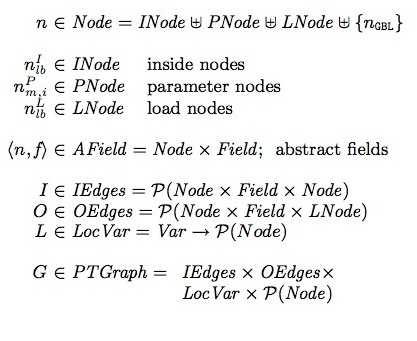
\includegraphics[width=0.5\textwidth]{data-representation}
  \caption{Representaton of data as presented in the paper}
\end{center}
\end{figure}

\subsubsection*{Algorithm}

As presented in the paper the algorithm consists of an intra- and
inter-procedural analysis. This separation, however, is largely
fictional as the inter-procedural analysis uses the intra-procedural
analysis and vice versa. Using this separation does make it easier to
explain the algorithm so I'll carry on in the same spirit. \newline

The \textbf{intra-procedural} analysis constructs a points-to graph of
a single method without knowing the calling context and  when a method
invocation occurs, say, when $m1$ invokes $m2$ then the \textbf{inter-
procedural} analysis instantiate the  parameterized result of $m2$ and
use that in the analysis of $m1$. \newline

The algorithm processes the strongly connected components of the call
graph from the leaves to the main method. Using a work-list it invokes
the  intra-procedural analysis on each method in the strongly
connected components until a fixed-point is reached. \newline

The intra-procedural analysis is a forward-flow analysis and for each
statement it uses a transfer function that given a points-to graph and
a statement will compute the points-to graph right after the
statement. It also computes the set of modified abstract fields. For a
detailed description of each of the transfer functions see the paper.
\newline

The inter-procedural analysis does four things: 

\begin{itemize}
  \setlength{\itemsep}{1pt}
  \setlength{\parskip}{0pt}
  \item Constructs a node mapping from nodes of the points-to graph of 
        $m2$ ($G_{callee}$) to nodes of the points-to graph of 
        $m1$ ($G$). The node mapping disambiguates as many parameter- 
        and load-nodes from the callee as possible
  \item Combines the graph $G$ and graph $G_{callee}$
  \item Simplifies the resulting graph
  \item Updates the set of modified abstract field
\end{itemize}

\subsubsection*{Using the results}

Once the analysis is done we have a points-to graph for each method in
the program. We use these to derive information abut the
program. A \textbf{method is pure} if the set of modified abstract
fields is empty. If a method isn't pure we can infer a regular
expressions that describe all the pre-state locations modified by $m$.
This  is simply done by constructing a finite state automaton $F$ with
the following states:

\begin{itemize}
  \setlength{\itemsep}{1pt}
  \setlength{\parskip}{0pt}
  \item All the nodes from the points-to graph $G$
  \item An initial state s
  \item An accepting state t
\end{itemize}

And the following transitions: 

\begin{itemize}
  \setlength{\itemsep}{1pt}
  \setlength{\parskip}{0pt}
  \item Each outside edge from $G$ generates a transition in $F$ labeled with 
        the field of the outside edge
  \item For each parameter $p_i$ of $m$, we create a transition from $s$ to 
        the corresponding parameter node, and label it with the parameter $p_i$
  \item For each mutated abstract field $<n,f>$ add a transition from $n$ to the 
        accepting state $t$. Label it with the field $f$.
\end{itemize}

Now we can generate the regular expressions by recording the labels of
all paths from the start state to the accepting state.

\subsection{Implementation}

The implementation can be found in the file
\texttt{src/main/scala/dk/itu/sdg/analysis/Purity.scala} and the tests
can be found in
\texttt{src/test/scala/dk/itu/sdg/analysis/PurityTest.scala} and
\texttt{src/test/scala/dk/itu/sdg/analysis/RegExpGeneratorTest.scala}.
\newline

I will attempt to give a high-level overview of the implementation
covering the entry points and which pieces of code do what and. For a
deeper understanding of the implementation I suggest reading the code
and the paper side-by-side. \newline

\texttt{analysis(className: String, invokable: SJInvokable): Result}
is the main entry point to the analysis. \texttt{className} is the
name of the class that contains the method (this is only needed
because \texttt{SJInvokable} doesn't have a reference to the class in
which it is defined) and \texttt{invokable} is the method (or
constructor) that you want to analyze. \texttt{Result} is simply a
\texttt{case class} that contains the points-to graph of the method
and the set of modified abstract fields. This method takes care of
the fixed-point iteration when analyzing each of the strongly
connected components of the call graph. \newline

The method \texttt{bulkTransfer} takes care of analyzing a list of
consecutive \texttt{SJStatement}s. It simply traverses the statements
from top to bottom and uses the transfer functions to transform the
points-to graph on every statement on the way and (possibly) adding
AbstractField to the writes set. The object \texttt{TransferFunctions}
contains methods for each of the transfer functions as defined in the
paper. The \texttt{case class TFState} is used to model the state as
each of the statements are being processed. \newline

\texttt{mapping} creates the appropriate node-mapping used when two
points-to graphs needs to be merged and \texttt{combine} takes care of
the actual merging of the two graphs. \newline

No mutable state is used in the implementation.

\subsection{State of Completion}

Largely the implementation works. For each of the examples in the
paper the implementation is successful in detecting if a method is
pure or not. Currently the test \texttt{PurityAnalysisExample.flipAll}
fails but this is only because the modified path strings aren't being
compressed, see \ref{subsub:mp}

\subsubsection*{Points-to graph simplification}

The paper explain how to simplify the points-to graph after merging
two points-to graphs after a method invocation. The current
implementation doesn't do any of these simplifications. I have
prepared the method \texttt{simplify} but it's currently the identity
function.

\subsubsection*{Static Fields}

There are a couple of aspects of Java that the article covers but the
current implementation doesn't. These are:

\begin{itemize}
  \setlength{\itemsep}{1pt}
  \setlength{\parskip}{0pt}
  \item Arrays
  \item Unanalyzable methods, i.e. methods where we don't have access to the source.
  \item Static Fields
\end{itemize}

As I understand the two first points can be ignore in Kopitiam but the
third one might be of interest. I have implemented the transfer
functions related to static fields but due to a problem\footnote{See
the mail to Hannes in the appendix describing this error in some more
detail.} somewhere when the SimpleJava AST is being generated I
haven't been able to complete the implementation. I have, however,
added TODO comments in the code that describe what would need to be
changed.

\subsubsection*{Modified Paths}
\label{subsub:mp}

With the current implementation it's possible to generate string that
show the paths of the objects that are being modified (if any). I
still need to add some compression to the strings such that

\begin{itemize}
  \setlength{\itemsep}{1pt}
  \setlength{\parskip}{0pt}
  \item foo.bar.x
  \item foo.bar.y
  \item foo.bar.next.x
  \item foo.bar.next.y
  \item foo.bar.next.next.x
  \item foo.bar.next.next.y
\end{itemize}

turns into: \texttt{foo.bar.next*.(x|y)}

\subsection{Things not mentioned in the paper}

There is one thing that wasn't completely clear from the paper and one
thing that was neglected

\begin{itemize}
  \item When a statement is of the form \texttt{v = new C} then in 
        addition to invoking the transfer function as described in 
        the paper it should also be considered a method invocation.
  \item The article doesn't mention entirely how to deal with while loops 
        so I had to improvise: let \texttt{G} be the graph before the loop 
        iteration and let \texttt{G'} be the graph produced by the loop 
        iteration. Consider the \texttt{Edge(n1,f,n2)} from \texttt{G'} 
        that doesn't exist in \texttt{G}, i.e. an edge produced by the 
        iteration. If there exists an \texttt{Edge(n1,f,n3)} in \texttt{G} 
        then map the node \texttt{n2} to \texttt{n3}.
\end{itemize}

\newpage

\section{Possible Code Improvements For When There's More Than 24h In A Day}

This is a list of various possible improvements to the parts of the
code base of Kopitiam that I've worked on.

\subsection{Lenses}

In the purity analysis I use case classes to model the state of the
algorithm. In an effort to stay sane these case classes are all
immutable so I use the \texttt{copy} method when I need to make
changes to the data structure. However, this gets quites messy when I
want to change something deep in the data structure as shown below.

\begin{figure}[h!]
  \begin{lstlisting}
  state.copy(
    result = state.result.copy(
      pointsToGraph = ptGraph(state).copy(
        stateOflocalVars = localVars(state).updated(v1, nodes)
      )
    )
  )
  \end{lstlisting}
\end{figure}

This answer\footnote{http://stackoverflow.com/questions/3900307
/cleaner-way-to-update-nested-structures\#answer-5597750}  on Stack
Overflow contains information about lenses with references to a CS
paper and blog posts with examples in Scala. You could hand-code the
lenses for the appropriate case classes or if you're feeling brave use
this compiler plugin\footnote{https://github.com/gseitz/Lensed} that
generates them for you. \newline

With lenses you could change to code to something like this:

\begin{figure}[h!]
  \begin{lstlisting}
    state.result.pointsToGraph.stateOfLocalVars.mod(state, _.updated(v1, nodes ))
  \end{lstlisting}
\end{figure}

\subsection{Type-safe AST transformations}

Currently when we're transforming the AST during static analysis we're
using casting to make it compile. We could instead use the same
approach as they do in the Scala compiler\footnote{https://github.com/
scala/scala/blob/master/src/library/scala/reflect/api/Trees.scala\#L10
35} where we simply define a Transformer abstract class with methods
for each of the AST nodes we want to be able to rewrite. For a
specific rewrite of the tree we then create a new instance of
Transformer and override the tranformXXX method of the node we want to
work with. An example of this is shown in figure
\ref{transform_ast_scalac}.

\section{Appendix}

\begin{figure}[b]
\begin{lstlisting}
Hi Hannes,

FYI, the following example makes the AST transformation to SimpleJavaAST crash:

class Person {

 static String defaultName = "Mr. Default";

 String name;

 public Person(String s) {
   this.name = s;
 }
}

class AssignToStaticField {
 public void setDefaultName(String defaultName) {
   Person.defaultName = defaultName;
 }
}

I get the exception: java.util.NoSuchElementException: key not found: Person

And it's because of the line: Person.defaultName = defaultName;

You can invoke this by running:

test-only dk.itu.sdg.analysis.PurityTestsByMads

or

run src/test/resources/static_analysis/source/AssignToStaticField.java

and hit 1.
\end{lstlisting}
  \caption{Mail to Hannes describing error in the AST transformation to SimpleJava AST}
  \label{mail_to_hannes}
\end{figure}

\begin{figure}[b]
\begin{lstlisting}
object Test {

  def main(args: Array[String]): Unit = {
    abstract class Transformer {

      def transform(defi: Definition): Class = defi match {
        case Class(name, body) => Class(transformName(name), body map {transformStatement(_)})
      }

      def transformName(name: String): String = name

      def transformValue(value: Int): Int = value

      def transformStatement(stm: Statement): Statement = stm match {
        case VariableWrite(id, value) => VariableWrite(transformName(id), transformExpression(value))
        case Return(expr) => Return(transformExpression(expr))
      }

      def transformExpression(exp: Expression): Expression = exp match {
        case VariableAccess(id) => VariableAccess(transformName(id))
        case Value(value) => Value(transformValue(value))
      }
    }

    // AST definition
    sealed trait Transformable
    sealed trait Definition extends Transformable
    case class Class(name: String, body: List[Statement]) extends Definition

    sealed trait Statement extends Transformable
    case class VariableWrite(id: String, value: Expression) extends Statement
    case class Return(expr: Expression) extends Statement

    sealed trait Expression extends Transformable
    case class VariableAccess(id: String) extends Expression
    case class Value(value: Int) extends Expression

    // Build a simple test AST
    val ast = Class("Thingy", List(
      VariableWrite("foo", Value(42)),
      Return(VariableAccess("foo"))
    ))

    // Do some transformations.
    println((new Transformer {
      override def transformName(name: String): String = name.reverse
      override def transformValue(value: Int): Int = value + 10
    }) transform ast)
  }
}
\end{lstlisting}
  \caption{Possible solution to type-safe tree re-write}
  \label{transform_ast_scalac}
\end{figure}

\end{document}